\chapter{PyBEL: a computational framework for Biological Expression Language}
\label{ch:pybel}

\section*{Preface}

While \ac{BEL} had been previously demonstrated to support the combination of data and knowledge in analyses~\cite{Martin2012,Laifenfeld2012,Catlett2013,Martin2014,Vasilyev2014,Laifenfeld2014}, manual curation and disease modeling~\cite{Kodamullil2015,Irin2015,Naz2016,Karki2017,Emon2017,Domingo-Fernandez2017}, and storage of biomedical text mining results~\cite{Lai2016,Madan2016,Rastegar-Mojarad2016,Ravikumar2017,Ali2017}; its surrounding computational ecosystem was incredibly limited.

The previously existing software provided by Selventa, the original developer of BEL, was aging and not amenable to extension or interactive computational investigation that is becoming mainstream with the advent of the Jupyter Notebook~\cite{Kluyver2016}.
In order to leverage the unique ability of \ac{BEL} to integrate multi-scale and multi-modal knowledge to support downstream simulation, target prioritization, mechanism of action deconvolution, and other methods, it was necessary to build a new ecosystem that is presented in the following publication.

\vspace*{\fill}

Reprinted with permission from "Hoyt, C. T., Konotopez, A., \& Ebeling, C. (2017) PyBEL: a computational framework for Biological Expression Language. \textit{Bioinformatics (Oxford, England)}, 34(4), 703–704".
Copyright © Hoyt, C.T., \textit{et al.}, 2017.

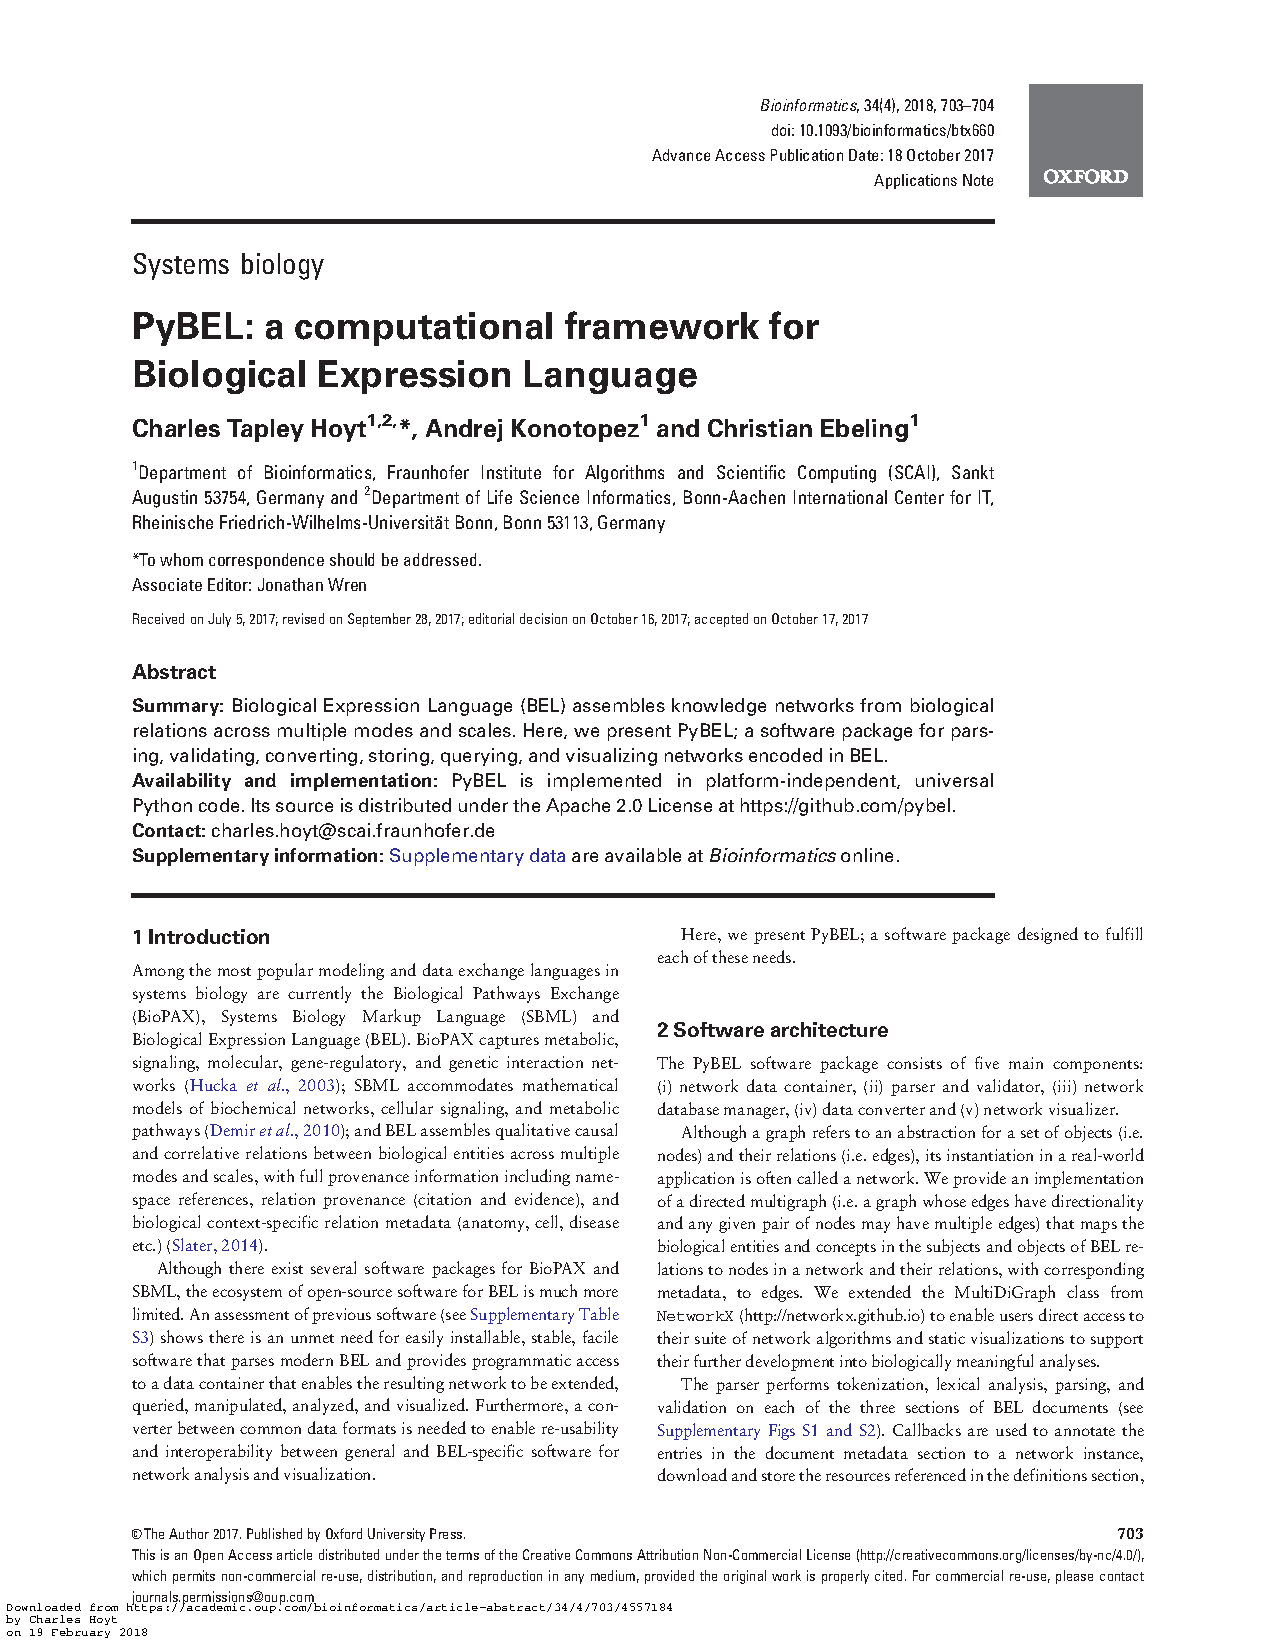
\includepdf[pages={-}]{articles/pybel.pdf}

\section*{Postface}

In order to make the PyBEL ecosystem sustainable, it was made open source, easily installable, integrated with existing systems in systems and networks biology, tested, and well-documented.
It was then demonstrated the ease with which \ac{BEL} could be used in the Python environment as well as presented an implementation of a variant of the heat diffusion algorithm described by~\cite{Leiserson2015}.

While PyBEL contained several imports and exports for other software used by systems and network biologists, it still lacked an accessible interface for biologists.
It was also alluded that knowledge from structured sources could be integrated, especially from other standards like \ac{BioPAX} and \ac{SBML}.
Each of these are addressed in Chapters~\ref{ch:belcommons}, ~\ref{ch:recuration}, and~\ref{ch:bio2bel}.

The goal of an academic thesis is not to highlight the projects from which the research came and was then used, but it would be remiss of me not to mention the number of places where PyBEL has been, and continues to be used, which have both caused me both great joy and great frustration as its maintainer.

PyBEL was originally developed in the Fraunhofer SCAI Department of Bioinformatics for usage in the \ac{IMI} project, AETIONOMY\footnote{\url{https://www.aetionomy.eu/}}, to support the generation of a taxonomy of mechanisms underlying neurodegenerative diseases such as Alzheimer's disease, Parkinson's disease, and epilepsy as well as patient stratification.
One of the project's major deliverables, NeuroMMSig~\cite{Domingo-Fernandez2017} was originally built with an ad-hoc database, but the upcoming verison has converted to PyBEL to take advantage of its entire suite of tools.
Following AETIONOMY, PyBEL has also been used in the \ac{IMI} project, PHAGO\footnote{\url{https://www.phago.eu/}}, which focused on the role of the TREM2 and CD33 proteins in Alzheimer's disease~\cite{Ebeling2017}.

The Fraunhofer SCAI Department of Bioinformatics has relied on PyBEL for the compilation, validation, and summarization of manually curated BEL documents in several internal and industry projects.
Three industry projects with Cohen Veterans Bioscience used PyBEL during the manual curation of causal and mechanistic knowledge related to post-traumatic stress disorder and traumatic brain injury.
One industry project with Boehringer Ingelheim focused on the manual curation of causal and mechanistic knowledge related to several psychiatric conditions such as depression and anhedonia.
The visualization tools developed during this project became the basis for BEL Commons, presented in Chapter~\ref{ch:belcommons}, that are also being reused in the Horizon 2020 project, VirtualBrainCloud\footnote{\url{https://www.scai.fraunhofer.de/de/geschaeftsfelder/bioinformatik/projekte/Virtual_Brain_Cloud.html}}.
An academic project with the Cytoscape Consortium\footnote{\url{http://www.cytoscapeconsortium.org}} focused on the integration of PyBEL with NDEx~\cite{Pratt2015} such that BEL documents could be uploaded and handled in NDEx using its CX format, as well as to enhance interoperability of both \ac{BEL} and CX with \ac{RDF}.
An internally funded project, The Human Brain Pharmacome Project\footnote{\url{https://pharmacome.scai.fraunhofer.de}}, has relied on PyBEL for compilation and analysis of BEL documents related to tauopathies and later more general neurodegenerative disease phenomena.
An internally funded project at the Fraunhofer Center for Machine Learning has used PyBEL as a source of biomedical triples for the training of network representation learning models in the bio2vec\footnote{https://bio2vec.net} project and resulted in the following publication~\cite{Ali2019}.
A project granted by the Human Brain Project, Reference Ontology Hub with Application services for Neurosciences (ROHAN)\footnote{\url{https://www.scai.fraunhofer.de/en/business-research-areas/bioinformatics/projects/Rohan.html}} has used the terminology mangement functions of PyBEL that later became Bio2BEL.

PyBEL has been used by external groups, including several pharmaceutial companies part of the AETIONOMY project as well as interest from Clarivate Analytics, who provide their Metacore\footnote{\url{https://clarivate.com/products/metacore/}} knowledge bases as BEL to customers.

Finally, PyBEL has been used in several publications and theses by other members of the Fraunhofer SCAI Department of Bioinformatics~\cite{Domingo-Fernandez2018,Domingo-Fernandez2019a,Mubeen2019} as well as slow uptake by the broader community of systems and network biologists~\cite{Kwon2019,Gyori2017} and further upcoming masters and doctoral theses.
